\chapter{Related Work}
Low-light image enhancement methods have been widely developed to obtain high-contrast images in the field of consumer imaging devices. Recently, the performance of low-light image enhancement has become an important quality measure of recent consumer imaging devices. Although recent consumer imaging devices increase the size of the aperture to acquire a brighter image, the low sensitivity of an imaging
sensor under low-light condition results in the low signal-to-noise ratio (SNR). As a result, the low-light enhanced image cannot avoid the unnatural artifacts such as noise amplification and color distortion. An image is an array, or a matrix, of square pixels (picture elements) arranged in columns and rows .An Image is a 2D function f(x, y) , where x and y are spatial coordinates and amplitude of f at any pair of coordinates (x, y) is called the intensity or gray level of the image.

To enhance the contrast of a low-light image, histogram-based methods adjust pixel values using the cumulative distribution function (CDF) of the input image. Chen et al. redistributed the intensity bins of multiply divided sub-histograms [1]. However, since the histogram of a low-light image is extremely narrow, the resulting image shows noise amplification and the saturation in the bright region. To solve this problem, Gu et al.proposed a variational contrast enhancement framework by minimizing the constraint terms on the histograms using $l_{2}$ -norm . They automatically selected the regularization parameter according to the assessed score of the image quality
measure.

\section{Digital Image Processing}
In terms of low-light video enhancement, Ko et al. proposed a temporal flicker-free low-light video enhancement method [5]. This method enhanced input low-light video by accumulating the similar patches in the specified searching region among temporally adjacent frames. However, the resulting image shows the blocking artifact since the mean brightness value may vary indifferent patches because of gamma correction. Kim et al. enhanced the low-light video using the clipped histogram stretching on each color channel and performed the spatio-temporal noise reduction under the non-local means filter framework at the high-computational cost [6]. Image processing is a method to perform some operations on an image, in order to get an enhanced image or to extract some useful information from it. It is a type of signal processing in which input is an image and output may be image or characteristics/features associated with that image. Nowadays, image processing is among rapidly growing technologies.Image processing basically includes the following three steps:
\begin{itemize}
	\item Importing the image via image acquisition tools;
	\item Analysing and manipulating the image;
	\item Output in which result can be altered image or report that is based on image analysis.  
\end{itemize}

\subsection{Light and visible spectrum}
If a beam of white light passes through a glass prism, the human can see that the beam of light is broken and the six colors of the spectrum appear: red, orange, yellow, green, blue and violet (Figure\ref{fig:colorSpectrum}). This is known as refraction and was discovered by Sir Isaac Newton in 1666. In this way, you can understand that white light, existing everywhere, is composed of a spectrum of colors and collided with a body, it absorbs any of these components and reflects others. The reflected colors are what our eyes can perceive \cite{dip1}.
\begin{figure}
  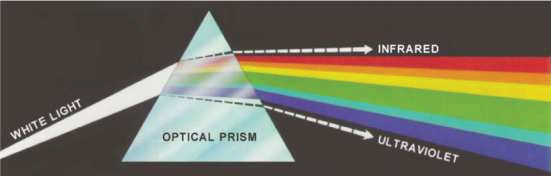
\includegraphics[width=\linewidth]{images/ch2/colorSpectrum.jpg}
  \caption{Color spectrum seen by passing White light through a prism}
  \label{fig:colorSpectrum}
\end{figure}

Basically, the colors that human perceive depend on the nature of the light reflected from the object. So the visible range by human eyes can be seen (Figure \ref{fig:wavelength}) as a little part within the electromagnetic spectrum and include wavelengths from 380 nm to 780 nm. The human eye perceives light from each of these wavelengths as a different color\cite{dip1}.


\begin{figure}
  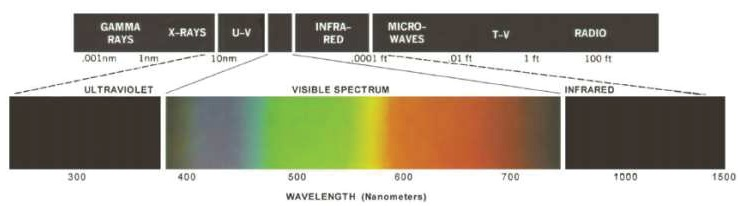
\includegraphics[width=\linewidth]{images/ch2/wavelength.jpg}
  \caption{Wavelengths comprising the visible range of the electromagnetic spectrum}
  \label{fig:wavelength}
\end{figure}

Primary color is a color that cannot be obtained by mixing any other one. This is an idealized model, based on the biological response of the receptor cells of the human eye (cones) in the presence of certain frequencies of light and noise, and is dependent on the subjective perception of the human brain. Mixing two primary colors gives rise to a secondary color \cite{dip1}.
The theories of traditional and modern color disagree on which are the primary colors. The modern color theory distinguishes between light and pigment colors (Figure \ref{fig:mixtureLight},Figure \ref{fig:mixturepigment}) \cite{dip2}.

\begin{itemize}
	\item Light primary colors (RGB model): Red, green and blue.
	\item Primary pigment colors (CMY Model): Cyan, magenta and yellow.
	\item Traditional primary colors (RYB Model): Red, yellow and blue.This model is the precursor CMY model. It is considered obsolete by science and industry.
 
\end{itemize}

It is called secondary when a color is obtained by mixing two primary colors and which in turn is complementary color of a third primary color, which is not involved in its preparation\cite{dip1,dip2}.

\begin{itemize}
	\item Secondary colors light (RGB model) and Cyan, magenta yellow
	\item  Secondary colors pigment (CMY Model): Orange, green and violet.
\end{itemize}

\begin{figure}
  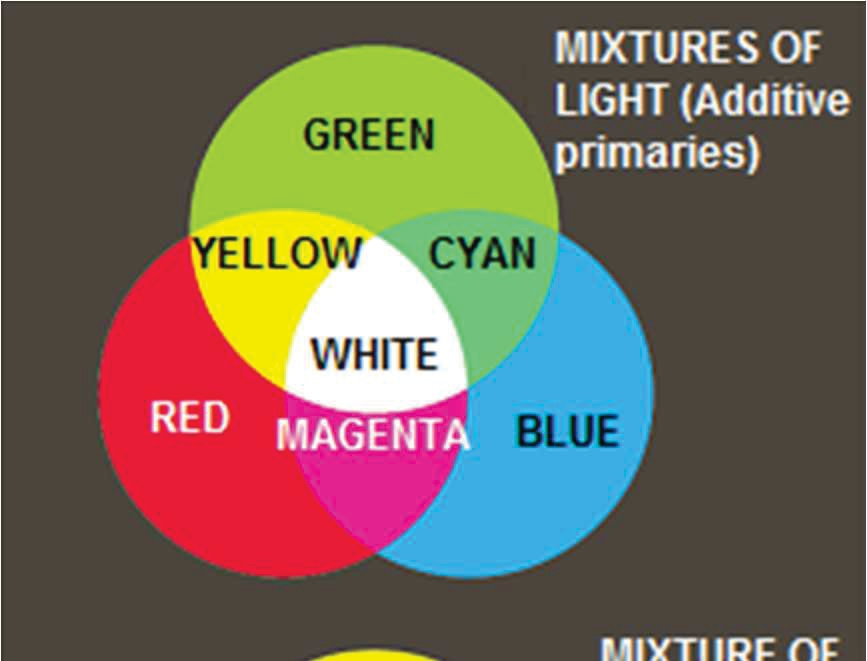
\includegraphics[width=\linewidth]{images/ch2/mixtureLight.jpg}
  \caption{Primary and secondary colors of light}
  \label{fig:mixtureLight}
\end{figure}

\begin{figure}
  \includegraphics[width=\linewidth]{images/ch2/mixturepigment.jpg}
  \caption{Primary and secondary colors of pigments}
  \label{fig:mixturepigment}
\end{figure}


\subsection{Digital image}
The term image refers to a two dimensional function of light intensity f (x, y) where x and y denote the spatial coordinates and the value of f at any point (x, y) is proportional to the intensity of the image at that point \cite{dip2}. A digital image can be written as a matrix whose row and column indices identify a point in the image and whose value coincides with the level of light intensity at that point. Each element of the array corresponds to an element in the image and is called pixel\cite{dip1}

\begin{equation}
	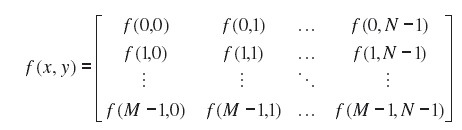
\includegraphics[scale=1]{images/ch2/imageMatrix.jpg}
	\label{eq:imageMatrix}
\end{equation}

The notation of coordinates widely accepted by most of the books is shown in equation (\eqref{eq:imageMatrix}) where the image has M rows and N columns determining the origin at the point f (0,0).

Figure \ref{fig:leena} shows four version of the same picture where the difference is the number of pixels in each of them. This means that the pixel is only one division unit without a particular actual size. Only when the image resolution is given, a particular size to the pixel is assigned\cite{dip4}.
\begin{figure}
  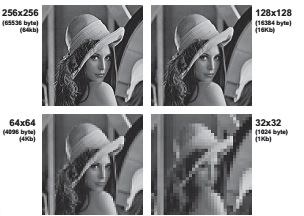
\includegraphics[width=\linewidth]{images/ch2/leena.jpg}
  \caption{Digital Image of "Lenna" with different number of pixels}
  \label{fig:leena}
\end{figure}

\subsection{Classification of digital image}
There are many kind of classification of digital image. A Basic classification should be: bitmap and vector images. Vector images are obtained based on lines, each responding to a mathematical equation. An image of this type is formed by controlled strokes coordinates. Vector graphics have the disadvantage that they do not have the level of detail of bitmaps. The advantage is that you can reduce and enlarge without losing quality since the lines are redrawn when resizing \cite{dip1}.
Bitmap images were described in point 2.1.2. These kinds of images are used in this project. Figure \ref{fig:vectorAndBitmap} shows differences between bitmap and vector images

\begin{figure}
  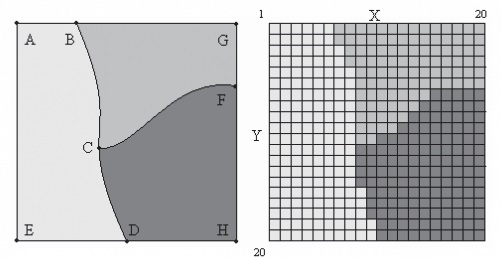
\includegraphics[width=\linewidth]{images/ch2/vectorAndBitmap.jpg}
  \caption{a) Vector and b) bitmap images}
  \label{fig:vectorAndBitmap}
\end{figure}

\subsection{Color spaces}
Color spaces are a defined range of colors that in combination with physical device, it allows representations of color in analog and digital way.A color model is an abstract mathematical model describing the way colors can be represented as tuples of numbers \cite{dip3}.

There are many types of model color but only the first 3 are important in this project.

\begin{itemize}
	\item Grayscale
	\item RGB
	\item HSV
	\item Others: YCbCr, HLS, CMY, etc.
\end{itemize}

\subsubsection{Grayscale}
An intensity scale is also known as monochrome or grayscale level and to a digital image is an MxN array of values where each pixel is a single sample containing the information of the image intensity\cite{dip4}. In a grayscale image(figure \ref{fig:grayScaleImage}) each pixel has a brightness value between 0 (black) to 1 (white). Commonly, this mode uses up to 256 shades of gray (8 bits per sampled pixel). Another way of representation is as percentage. The 3 characteristics that can define a color are hue (color), value (lightness or darkening) and saturation (color purity) \cite{dip4}. Thus the conversion of a color image to a grayscale image is not performed in a unique way, however in its most common approach\cite{dip3}, it is to retain information on the brightness and discard the values of hue and saturation. Assuming the colors red, green and blue are signs of light, the approximation of an image in grayscale from a color image is given by equation (\ref{eq:gray}) where 0 is the value of less intensity, referring to the color black and 1 is the value of greater brightness or white \cite{dip4}.

\begin{equation}
	GRAY = (0.30 \cdot R) + (0.59 \cdot G) + (0.11 \cdot B)
	\label{eq:gray}
\end{equation}

\begin{figure}
	\begin{subfigure}{6cm}
		\centering    
    	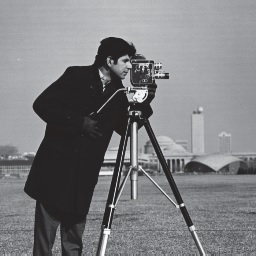
\includegraphics[width=7cm,height=9cm,keepaspectratio]{images/ch2/grayScaleImage.jpg}
    \end{subfigure}
  	\begin{subfigure}{6cm}
  		\centering
  		
\includegraphics[width=4cm,height=7cm,keepaspectratio]{images/ch2/grayLevelImage.jpg}
   
  	\end{subfigure}
  	\centering\caption{a) Greyscale images y b) Grey levels of greyscale images}
  	\label{fig:grayScaleImage}
\end{figure}

\subsubsection{RGB model}
An RGB image is defined as an array of 3xMxN pixels where each pixel corresponds to the red, green and blue components of a color image. The main purpose of the RGB model is the sensing, representation and display of images in electronic devices such as televisions, computers, cell phones, etc \cite{dip3}.

The RGB model can be viewed as a stack of 3 scale image intensities to be displayed on a color monitor (which has 3 color inputs, red, green and blue). Colors red, green and blue are known as primary colors, and the combination of these different intensities in colors produces human visible spectrum. Figures \ref{fig:RGBColorCube} show a 3D representation of the RGB model \cite{dip4}.

Generally the intensity of each of the components is measured on a scale from 0 to 255 (1 byte per component)

\begin{figure}
	\centering  
  	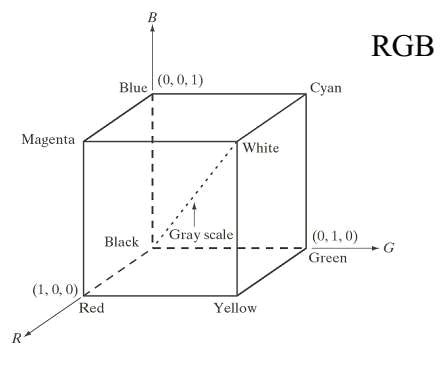
\includegraphics[scale=1]{images/ch2/RGBColorCube.jpg}
  	\caption{Schematic of the RGB color cube. Points along the main diagonal have gray values, from black at the origin to white at point (1,1,1)}
  	\label{fig:RGBColorCube}
\end{figure}

\begin{figure}
	\centering
  	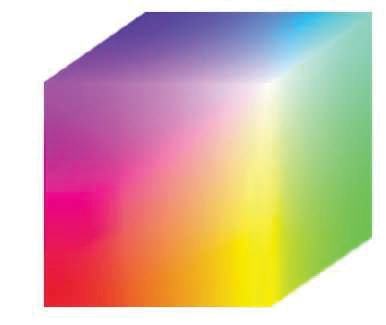
\includegraphics[scale=0.8]{images/ch2/RGB24ColorCube.jpg}
  	\caption{RGB 24-bits color cube}
  	\label{fig:RGBColorCube}
\end{figure}
This model is the most used to display digital images on a screen in the current formats so it is very important in the image processing\cite{dip4}

\subsubsection{HSV model}
The HSV model is based on the human perception of color and describes, according to CIE [quote]:
\begin{itemize}
	\item Hue: The "attribute of a visual sensation according to which an area appears to be similar to one of the perceived colors: red, yellow, green, and blue, or to a combination of two of them".
	\item Saturation: Colorfulness of an area judged in proportion to its brightness.
\end{itemize}
The HSV color model is based in the RGB model, but it is a cylindrical coordinate model. It uses the following three components [9]

\begin{itemize}
	\item H (hue) is usually represented in a circumference, so the degree says the color of that pixel, but it is also used in a percentage way for some applications.
	\item S (saturation), the representation of this component is the distance from the cylinder axe.
	\item V (value, also called B, brightness), this is the component used in the transform. Usually, it is represented from 0 to 1 (also in Matlab). If the value is 0, it means that the pixel is black, regardless of the other two components (for this reason, the HSV model can also be interpreted and represented like a cone) (figure \ref{fig:HSVModel}) \cite{dip4}.

\end{itemize}

\begin{figure}
	\centering
  	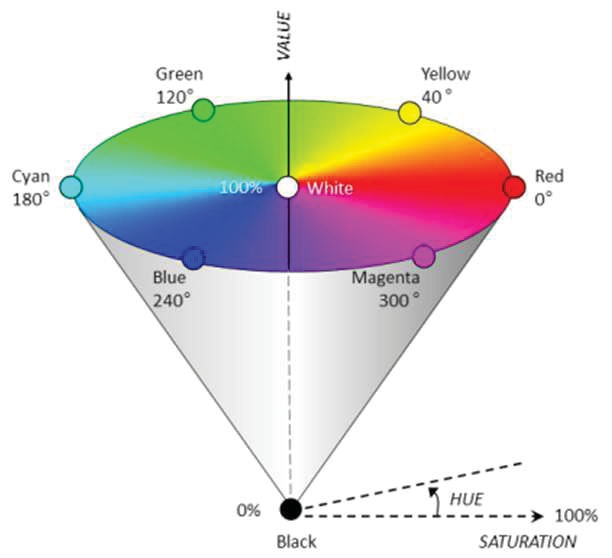
\includegraphics[scale=0.5]{images/ch2/HSVModel.jpg}
  	\caption{Cone of HSV model}
  	\label{fig:HSVModel}
\end{figure}

The transformation from RGB to HSV is given by:

\begin{figure}
  	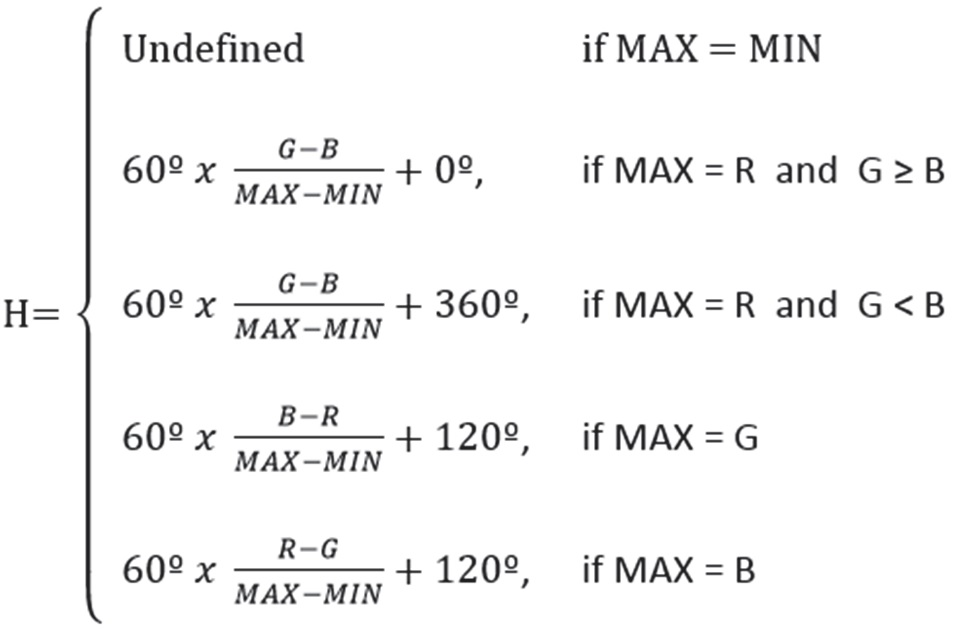
\includegraphics[scale=0.4]{images/ch2/H.jpg}
  	\label{fig:H}
\end{figure}

\begin{figure}
  	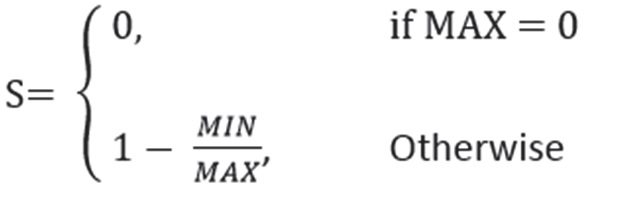
\includegraphics[scale=0.4]{images/ch2/S.jpg}
  	\label{fig:S}
\end{figure}

\begin{equation}
	V=MAX
\end{equation}

Hence, the formula indicates that for a pixel, the Value or Brightness is the maximum value of any of the RGB components. For example, if R is 0.7, G is 0.5 and B is 0.1 (normalized), the value for this pixel is 0.7.

\begin{figure}
	\begin{subfigure}{7cm}  
    	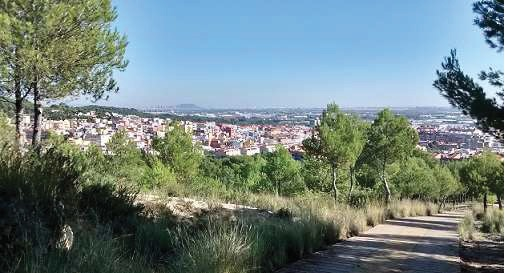
\includegraphics[width=7cm,height=12cm,keepaspectratio]{images/ch2/image.jpg}
    \end{subfigure}
  	\begin{subfigure}{5cm}
  		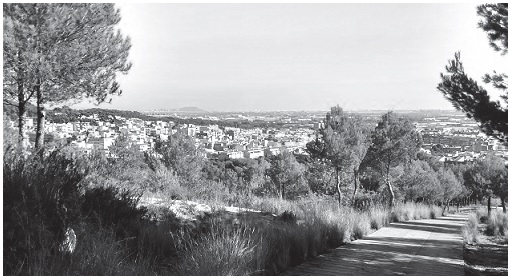
\includegraphics[width=7cm,height=12cm,keepaspectratio]{images/ch2/brightness.jpg}
   
  	\end{subfigure}
  	\caption{a) Original picture. b) Component brightness of original picture}
  	\label{fig:image}
\end{figure}


\subsection{Digital Image processing}
The digital image processing is the set of techniques applied to digital images in order to improve quality or facilitate the search for information \cite{dip1}.

The field that handles the processing of digital images is the digital image processing. Most processing techniques act treating the image as a two dimensions signal and then applying standard signal processing techniques of one dimension. Among the most common processing operations are\cite{dip2}:
\subsubsection{Intensity Transformation}
Exists for the spatial domain techniques that operate directly on the image pixels. The processes discussed in this report are denoted by the expression
\begin{equation}
	 g(x,y) = T[f(x,y)]
\end{equation}
where the function f(x,y) is the input image, g(x,y) is the output image (processed image) and T is an operator on f, which is an operator defined in a specific neighborhood (x,y) on a point (x,y).

Knowing that the main space to define neighborhoods about some point (x,y) approach is to use a square or rectangular region centered at (x,y) as shown below in the following scheme.

\begin{figure}
	\centering
		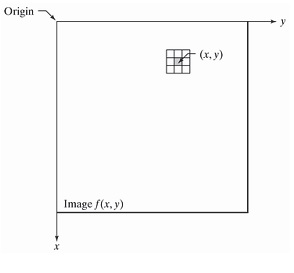
\includegraphics[scale=1]{images/ch2/spatialDomain.jpg}
		\caption{Spatial Domain}
		\label{fig:spatialDomain}
\end{figure}

The way to do this is to move starting pixel by pixel, that is, starting from the upper left corner as it moves, different neighborhoods are included. The operator T is applied to each location (x,y) thus g output can be obtained at that location. Only the pixels in the neighborhood are used to calculate the value of g(x,y).

Intensity transformation functions; the simplest form of the transformation T is when the neighborhood size is 1x1 (one pixel). In this case, the value of g(x,y) depends only on the intensity at that point f, and T becomes a transformation function intensities or gray Levels \cite{dip2}. As depend only on the intensity values, and not explicitly on (x,y), these functions are usually written in simplified form as;

\[
	s=T(r)
\]
Where r denotes the intensity of f and s the intensity of g, both on a corresponding point (x,y) of the image [4].

Some of these techniques are;

\begin{itemize}
	\item Linear
		\begin{itemize}
			\item Negative; Invert the order of the intensity values. 
				\[
					T(r){=}L-1-r
				\]
			\item Brightness; change of the average intensity of the image 
				\[
					T(r)=r \pm B 				
				\]	
				(B is real number)
			\item Contrast; change of the dynamic range of the image. 
				\[
					T(r)=r \cdot B 
				\]		
				(B is real number)
				\begin{figure}
					\centering
					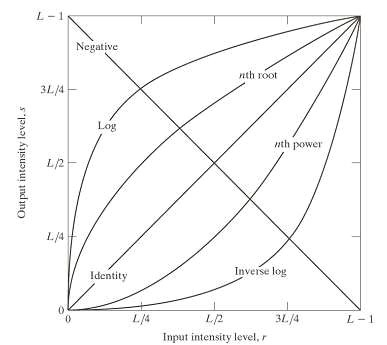
\includegraphics[scale=1]{images/ch2/basicTransformation.jpg}
					\caption{Basic transformations}
					\label{fig:basicTransformation}
				\end{figure}						
		\end{itemize}
		\item Nonlinear;
			\begin{itemize}
				\item Log; It is used to display low levels of intensity with greater dynamic range.
					\[
						T(r)=c log(1+r)
					\]
				\item Log power-law; It is similar to the log transformation. The advantage is the variety of  transformations to modify the value of n 
					\[
						T(r)=c \thinspace r^n
					\]									
				\item Histogram equalization;	
			\end{itemize}			
		\item Thresholding;
			\begin{itemize}
				\item change a gray scale image in binary image (black and white) through a threshold
					\[
						T(r)=
							\begin{cases}
								0,&if r \textless T\\
								255,&if r \textgreater T
							\end{cases}
					\]
			\end{itemize}
\end{itemize}

\subsubsection{Geometric transformation;}
Geometric transformation modify the spatial relationship between pixels. In terms of digital image processing a geometric transformation consists of two basic operations \cite{dip4}:				

\begin{itemize}
	\item A spatial transformation that defines the relocation of the pixels in the image plane.
	\item Interpolation of gray levels, which are related to mapping the intensity values of the pixels in the transformed image.
\end{itemize}

\subsubsection{Transformations into frequency domain}
\begin{itemize}
	\item Fourier Transformation
	\item Filter
\end{itemize}
for this project,intensity transformation is used.


\subsection{Image Enhancement}
The main definition of enhancing is to make something greater in value, desirability or attractiveness. The term of enhancement implies a process to improve the visual quality of the image \cite{ie1}. Image Enhancement transforms images to provide better representation of the subtle details. The principal objective of enhancement is to process an image so that the result is more suitable than the original image for a specific application\cite{lime}. Image enhancement processes consist of a collection of techniques that seek to improve the visual appearance of an image or to convert the image to a form better suited for analysis by a human or a machine. In an image enhancement system, there is no conscious effort to improve the fidelity of a reproduced image with regard to some ideal form of the image, as is done in image restoration \cite{lime}.

Actually, there is some evidence to indicate that often a distorted image, for example, an image with amplitude overshoot and undershoot about its object edges, is more subjectively pleasing than a perfectly reproduced original\cite{ie2}. Enhancement of an image is necessary to improve appearance or to highlight some aspect of the image is converted from one into another acquired, scanned, transmitted, copied or printed many types of noise can be present in the image. Image enhancement has come to specifically mean a process of smothering irregularities or noise that has somehow corrupted the image. The term “image enhancement” has been widely used in the past to describe any operation that improves image quality by some criteria. However, in the recent years the meaning of the term has evolved to denote image-preserving noise smoothing\cite{lime}.

This primarily serves to distinguish it from similar-sounding terms, such as image restoration and image reconstruction, which also taking specific meaning\cite{lime2}. Image enhancement has played and will continue to play an important role into different fields such as medical, industrial, military and scientific applications. In addition to these applications, image enhancement is increasingly being used in consumer electronics\cite{ie1}. Internet Web users, for instance, not only rely on built-in image processing protocols such as JPEG (Joint Photographic Expert Group) and interpolation, but they also have become image processing users equipped with powerful yet inexpensive software such as Photoshop. Users not only retrieve digital images from the Web but they are now able to acquire their own by use of digital cameras or through digitization services. Image enhancement is an indispensable tool for researchers in a wide variety of fields \cite{colorSpace2}:
\begin{itemize}
	\item In forensics, image enhancement is used for identification, evidence gathering and surveillance. Images obtained from fingerprint detection, security videos analysis and crime scene investigations are enhanced to help in identification of culprits and protection of victims.
	\item In atmospheric sciences IE is used to reduce the effects of haze, fog, mist and turbulent weather for meteorological observations. It helps in detecting shape and structure of remote objects in environment sensing. Satellite images undergo image restoration and enhancement to remove noise.
	\item Astrophotography faces challenges due to light and noise pollution that can be minimized by IE. For real time sharpening and contrast enhancement several cameras have in-built IE functions. Moreover, numerous softwares allow editing such images to provide better and bright results.
	\item In oceanography the study of images reveals interesting features of water flow, remains concentration, geomorphology and bathymetric patterns to name a few. These features are more clearly observable in images that are digitally enhanced to overcome the problem of moving targets, deficiency of light and obscure surroundings.
	\item IE techniques when applied to pictures and videos help the visually impaired in reading small print, using computers and television and face recognition. Several studies have been conducted that highlight the need and value of using IE for the visually impaired.
	\item The technique of image enhancement is often employed by virtual restoration of historic paintings and artifacts in order to reduce stains and crevices. Color contrast enhancement, sharpening and brightening are just some of the techniques used to make the images bright. IE is a powerful tool for restorers who can inform decisions by viewing the results of restoring a painting beforehand. It is evenly useful in discerning text from worn-out historic documents.
	\item In the field of e-learning, IE is used to clarify the contents of chalkboard as viewed on streamed video; it improves the content readability and helps students to focus on the text.Similarly, collaboration through the whiteboard is facilitated by enhancing the shared data and diminishing artifacts like shadows and blemishes.
	\item Medical imaging uses IE techniques for reducing noise and sharpening details to improve the visual representation of the image. Since minute details play a critical role in diagnosis and treatment of disease, it is essential to highlight important features while displaying medical images. This makes IE a necessary aiding tool for viewing anatomic areas in MRI, ultrasound and x-rays to name a few.
	\item Numerous other fields including law enforcement, microbiology, biomedicine, bacteriology, climatology, meteorology, etc., benefit from various IE techniques. These benefits are not limited to professional studies and businesses but extend to the common users who employ IE to cosmetically enhance and correct their images.
	
\end{itemize}

The following image(figure \ref{fig:imageEnhancementTechniques} explains the different types of image enhancement techniques.

\begin{figure}
	\centering
	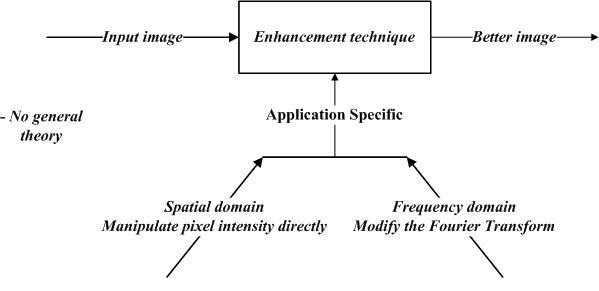
\includegraphics[scale=0.7]{images/ch2/imageEnhancementTechniques.jpg}
	\caption{Image enhancement techniques}
	\label{fig:imageEnhancementTechniques}
\end{figure}

In this project, spatial domain is considered.



%\begin{table}[h!]
%	\begin{center}
%	\caption{Techniques and Features.}
%    \label{tab:table1}
%	\begin{tabular}{ | m{4cm} | m{8cm}| }
%	\hline
%		Histogram Equalization & Adjusting the global contrast of an image. It is most effective method for gray scale images \\
%	\hline
%		Adaptive histogram Equalization & It is extension of HE and used within an image for local enhancement. It contains dark region and low contrast \\ 
%	\hline
%		Bi- histogram equalization & It maintains the intensity mean of the original image, which suppresses the over enhancement problem \\ 
%	\hline
%		Laplacian & It is mostly used for edge enhancement \\ 
%	\hline
%	\end{tabular}
%	\end{center}
%
%\end{table}

\subsection{Frequency Domain Technique}
Frequency domain method operates on the Fourier transform of an image. Image enhancement in the frequency domain is straightforward. We simply compute the Fourier transform of the image to be enhanced, multiply the result by a filter and take the inverse transform to produce the enhanced image. In frequency domain methods, the image is first transferred in to frequency domain\cite{ie1}. It means that, the Fourier Transform of the image is computed first. All the enhancement operations are performed on the Fourier transform of the image and then the Inverse Fourier transform is performed to get the resultant image\cite{lime3}. These enhancement operations are performed in order to modify the image brightness, contrast or the distribution of the grey levels. As a consequence the pixel value of the output image will be modified according to the transformation function applied on the input values [15]. The convolution theorem is the foundation of frequency domain techniques\cite{ie2}. Consider the following spatial domain operation:

\begin{equation}
	g(x,y)=h(x,y)*f(x,y)
\end{equation}

The following frequency domain relationship given by the convolution theorem 

\begin{equation}
	G (u, v) = H (u, v) F (U, v)
\end{equation}


Where g, f and h having Fourier transform G, H and F respectively. H is known as the transfer function of the process. Many image enhancement problems can be viewed in the form of the above equation. The main aim is to select a transfer function that changes the image in such a way that certain features of an image are enhanced\cite{ie1}. Examples: edge detection, noise removal.

There are mainly three types of filters
\begin{itemize}
	\item Low pass filter
	\item High pass filter
	\item Band pass filter

\end{itemize}

In Low-pass filtering, sharp transitions and edges in the gray levels of an image contribute significantly to the high frequency content of its Fourier Transform. By attenuating a specified range of high-frequency components in the frequency domain, blurring is achieved. Through Low-pass filtering this task is performed\cite{ie1}.

By High-pass filtering, Image sharpening can be achieved in the frequency domain. Low-frequency components will attenuated by high pass filter the without disturbing high frequency information\cite{ie1}.

Band-pass filtering is a method in which the reflectance and illumination components can be filtered independently. The illumination component of an image is generally classified by slow spatial variation on the other hand the reflectance component of an image tends to vary abruptly. These characteristics lead to associating the low frequencies of the Fourier transform of the natural log of an image with illumination and high frequencies with reflectance thus it is filtered individually\cite{lime3}.

\subsection{Comparison between Spatial Domain Technique And Frequency Domain Technique}
\begin{itemize}
	\item Spatial domain is manipulation of pixels of an image. It is the technique for changing the representation of an image and used in many field such as sharpening and smoothing images. Whereas Frequency domain is the manipulation of Fourier transforms to enhance an image and perform purely with convolution theorem and it is used in changing the position of an image. 
	\item The advantage of spatial domain technique is that it is simple to understand and the complexity of these techniques is very low which helps in real time implementation. Whereas Frequency domain technique having advantages which include low computation complexity, easy to view, manipulation of image’s frequency composition and the special transformed domain property is easily applicable.
	
\end{itemize}

The disadvantages of spatial domain technique is that it does not provides adequate robustness and perceivably. Whereas the disadvantage of Frequency Domain is that it cannot enhance properly every part of an image simultaneously and the automation of image enhancement is also very difficult. Table \ref{tab:table1} shows the areas where Spatial Domain technique and Frequency domain technique are applied.

\begin{table}[h!]
	\begin{center}
	\caption{Features of spatial domain and frequency domain techniques.}
    \label{tab:table1}
	\begin{tabular}{| m{5cm} | m{8cm}| }
	\hline
		\textbf{Techniques} & \textbf{Feature}\\
	\hline
		Spatial Domain technique & It is used to alter The gray level value Of individual pixels and hence the overall contrast of the entire image. It is not possible to selectively enhance edges or other required information effectively. \\
	\hline
		Frequency domain technique & It is used to Easily enhance edges And other subtle information because they are high frequency content and frequency domain operates on frequency content of an image. In this technique, all parts of  an  image  are  not enhanced in uniform manner \\ 
	
	\hline
	\end{tabular}
	\end{center}

\end{table}


%\section{BASICS OF RETINEX THEORY}
%Retinex is the theory of human color vision proposed by Edwin Land to account for color sensations in real scenes. Color constancy experiments showed that color does not correlate with receptor responses. In real scenes, the content of the entire image controls appearances. A triplet of L, M, S cone responses can appear any color. Land coined the word “Retinex” (the contraction of retina and cortex) to identify the spatial image processing responsible for color constancy. Further, he showed that color sensations are predicted by three lightnesses observed in long-, middle-, and short-wave illumination. Retinex is also used as the name of computer algorithms that mimic vision’s spatial interactions to calculate the lightnesses observed in complex scenes \cite{retinex}.
%
%\subsection{Overview}
%Edwin H. Land, the inventor of hundreds of film patents, was struck by experiments showing that color sensations in real complex images depend on scene content. Film responds to the light falling on each tiny local region. Land realized that vision’s mechanisms were very different from film. His early experiments studied the colors observed in red and white projections [1]. He realized color appearance required both the cone responses to a local region and the neural spatial processing of the rest of the scene. He proposed the Retinex Theory\cite{retinex}.
%
%Land coined the word Retinex to describe three independent spatial channels. In 1964 he wrote: “We would propose that all of the receptors with maximum sensitivity to the long-waves in the spectrum, for example, operate as a unit to form a complete record of long-wave stimuli from objects being observed. (For convenience of reference, let us call this suggested retinal-cerebral system a “retinex.”)” [2, 3, 4, 5]. It is the word that describes the mechanism that performs the comparison of scene information to create the array of sensations of lightness in three channels\cite{retinex}.
%
%
%\subsection{Cone Quanta Catch}
%Visible light falls on objects that reflect some of it to the eye. Color vision depends on the spectrum of the illumination falling on an object and the spectrum of its reflectance. The product of these spectra describes the light coming to the eye. There are three types of cones in normal observers that are called L for long-wave-, M for middle-wave-, and S for short-wave-sensitive cones. The receptors’ spectral sensitivities multiplied by the light falling on the retina determines the L, M, S cone responses, namely, the “quanta catch” of the cones. The cones convert the quanta catch to nerve signals that pass through many spatial comparisons in the visual system. The cone quanta catch is the important transition from the physics of light to the physiology of vision. However, it is just the first step in the process.
%
%Light passes through filters that determine the spectrum of each illumination falling on circular pieces of paper. The light coming to the eye from the papers is modified again by the reflectance spectra of the papers. Further, in this experiment there is no light coming from the black surrounds.
%On the left, there is a tungsten light source at the top. There is a filter that absorbs more middle-wave than long- and short-wave visible light (magenta arrows). The green circular paper reflects more middle-wave than long- and short-wave light. The light coming to the eye is the product of these spectra. The integrals of that light using the three cone spectral sensitivities determine the L, M, S quanta catch values.
%
%
%%\begin{figure}[h!]
% % 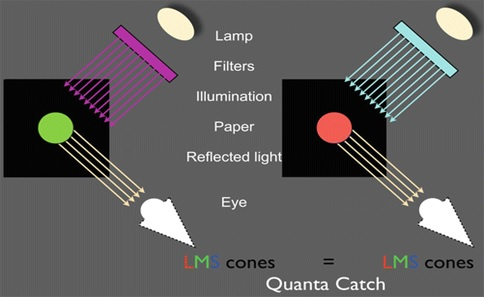
\includegraphics[width=1.7]{equalQuanta.jpg}
%  %\caption{equalQuanta}
%  	%\label{fig:equalQuanta}
%%\end{figure}
%
%%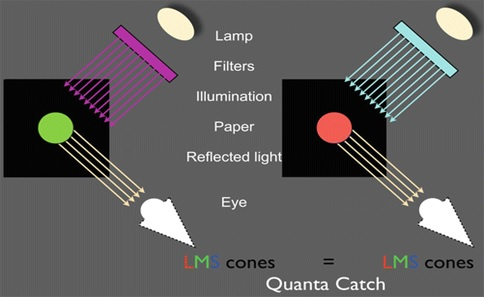
\includegraphics{{C:\Harish\Latex\Sample\equalQuanta.jpg}}
%
%On the right, there is the same tungsten light source at the top. There is a different filter that absorbs more long-wave than middle- and short-wave light (cyan arrows). The right-red paper reflects more long-wave than middle- and short-wave light. In this experiment, the spectra of the two illuminants and the two reflectances were adjusted to generate the same triplet of LMS cone quanta catches. Under these conditions, the left-green and right-red papers are identical retinal stimuli. They appear equal to each other, but that color is neither red nor green.
%
%\subsection{Mondrian Experiments}
%Land’s color Mondrian experiment is similar, with the exception that he used a complex array of papers to simulate real-world scenes. The important difference is that in complex scenes, a particular quanta catch can appear in any color: red, green, blue, yellow, white, or black.
%
%It used two identical Mondrians made of color papers, and three different, non-overlapping spectral illuminants (long-, middle-, and short-wave visible light). In this experiment observers reported the colors of papers in the Mondrians. In this illustration, we will look at the circular red and green papers. Land adjusted the illuminant mixtures of light from the two sets of three projectors. The same amounts of L, M, S light came from the green circle on the left as from the red circle on the right. First, he turned on just the long-wave lights. He adjusted the amounts of illumination on the left-green and right-red circles so the meter readings were equal. Then, he did the same for middle- and short-wave light. The left-green and right-red circles had equal quanta catches by the L, M, S cones.
%
%
%%\begin{figure}[h!]
% % \includegraphics[width=1.7]{landsExperiments.jpg}
%  %\caption{landsExperiments}
%  	%\label{fig:equalQuanta}
%%\end{figure}
%
%Two identical sets of matte colored papers, with separate L, M, S illuminating projectors with voltage transformers for control of the amount of light. Telephotometer readings were projected above the Mondrians. The experimenter separately measured the L, M, S radiances from a green circle in the left Mondrian. Then, he adjusted the L, M, S radiances from a red circle on the right Mondrian to be the same. Observers reported different red and green colors produced by identical light stimuli.
%
%In this complex scene, observers reported that equal quanta catches appeared green on the left and red on the right. Observers reported color constancy, namely, that the red paper looked red and the green paper looked green despite the identical cone quanta catch \cite{retinex}.
%
%Land repeated this experiment with all the Mondrian papers. A constant L, M, S quanta catch could generate any color sensation. The presence of the complex scene introduced more information to the visual system. The scene’s spatial content stimulated vision’s spatial image processing mechanisms to generate color constancy. The post-receptor visual processing plays a dominant role in color appearance in real scenes. Land’s word “Retinex” gave this spatial process a name. As well, he proposed a theoretical mechanism \cite{retinex}.
%
%\subsection{Retinex Mechanism}
%The pair of Mondrians in only long-wave light with more light on the left than on the right. Their appearances are nearly constant. This is a common observation: humans are insensitive to large changes in uniform illumination.
%
%%\begin{figure}[h!]
%%  \includegraphics[width=1.7]{landsExperiments.jpg}
%%  \caption{landsExperiments}
%%  	\label{fig:equalQuanta}
%%\end{figure}
%
%The left Mondrian has more illumination than the right. Observers report that the left set is slightly lighter than the right. Each corresponding area is nearly the same lightness in the left and right Mondrians as shown in Figure 2.3
%
%As illustrated in Figure 2.3, the left-green circle looked dark when it generated the same L cone quanta catch as the lighter right-red circle. Vision’s spatial image processing rendered the red and green papers with different lightnesses in long-wave light. The lightnesses are stable with large changes in overall illumination.
%
%Figure 2.4. illustrates the Mondrian viewed in only middle-wave light. The left-green circle now looks light and the right-red looks dark. In the experiment they had the same M cone quanta catch. Vision’s spatial image processing rendered the red and green papers with different and opposite lightnesses in Fig. 2.4.
%
%%\begin{figure}[h!]
% % \includegraphics[width=1.7]{landsExperiments.jpg}
%  %\caption{landsExperiments}
%  	%\label{fig:equalQuanta}
%%\end{figure}
%
%Now, the left Mondrian has less illumination than the right. In this wave band the pattern of lightnesses differs from that in long-wave light. That lightness pattern is indifferent to the amount of uniform illumination. Land adjusted the left side and right side illumination so that the circles had equal meter readings
%
%In summary, if the two Mondrians are side by side in the same band of wavelengths, but different overall intensities, the observers report nearly the same set of lightnesses at corresponding locations in the left and right Mondrians. However, one side is detectably lighter than the other. With large uniform changes in illumination, observers report nearly constant lightnesses of the individual papers.
%
%The left-green paper has more long-wave and less middle-wave illumination. The right-red paper has less long-wave and more middle-wave illumination. When adjusted, those adjustments in amount of illumination make the red and green papers have identical radiances. Those adjustments do not significantly alter the lightnesses of the areas in separate illumination. When viewing the Mondrian in combined illumination, in color, those changes in illumination do not change the color appearances of the red and green papers.
%
%
%These observations led Land to propose the Retinex theory. The triplet of apparent lightnesses, not cone quanta catches, determines the color appearance. Constant LMS lightnesses generate constant colors. That hypothesis led to a study of color appearances in L, M, S bands of light. Do all red colors have the same triplet of lightness appearances? Does a red color always look [light, dark, dark] in L, M, S light? Does a green always look [dark, light, dark]? Does color appearance always correlate with the triplet of L, M, S lightnesses?
%
%The experiment is easy. Find a red, a green, and a blue filter. Be sure that the filters exclude the other two-thirds of the spectra. With a green filter you should just see greens with different lightnesses. You should not see a mixture of greens and yellows and blues. If you do, you need a filter with a narrower band of transmission.
%
%Identify a group of red objects. Look at them sequentially through the L, M, S filters. Look at them in different ambient illuminations. Look at them at different times of the day. Look at them in sunlight and shadows. Red colors are always (light, dark, dark) in L, M, S light. The same dependence of the triplet of L, M, S lightnesses holds for all colors (Table 2.3). Lightness is the output of spatial image processing. It is the result of post-receptor spatial processing. That is why lightness does not correlate with cone quanta catch. However, color does correlate with three lightnesses in long-, middle-, and short-wave light.
%
%
%\begin{table}[h!]
%	\begin{center}
%	\caption{Correlation table of color appearances and the apparent lightnesses in L, M, 		S illumination.}
%    \label{tab:table1}
%	\begin{tabular}{| m{3cm} | m{3cm}|m{3cm}|m{3cm}| }
%	\hline
%		\textbf{Color Apperance} & \textbf{Apperance in L-Light} & \textbf{Apperance in M-Light} & \textbf{Apperance in S-Light}\\
%	\hline
%		Red & Light & Dark & Dark \\
%	\hline
%		Yellow & Light & Light & Dark \\ 
%	
%	\hline
%		Green & Dark & Light & Light \\ 
%	
%	\hline
%		Cyan & Dark & Light & light \\ 
%	
%	\hline
%		Black & Dark & Light & light \\ 
%	
%	\hline
%		Mangenta & Light & Dark & light \\ 
%	
%	\hline
%		White & Light & Light & light \\ 
%	\hline
%		Black & Dark & Dark & Dark \\ 
%	
%	\hline
%	\end{tabular}
%	\end{center}
%
%\end{table}
%
%Retinex theory predicts that the triplet of L, M, S lightnesses determines color. Colors are constant with changes in illumination because the triplet of lightnesses is nearly constant.
%
%Land’s observation still stands: The triplet of lightnesses correlates with color. The observation is important because a variety of different phenomena can influence lightness, such as simultaneous contrast, the Corn sweet effect, and assimilation. Regardless of the cause of the lightness changes, when two identical physical objects look different, color appearances correlate with their L, M, S lightnesses. In the color assimilation display (Fig. 2.5), there are two sets of nine red squares that have the same reflectance and appear the same (top left). However, if these red squares are surrounded by yellow and blue stripes, they look different (top center): the left red squares fall on top of the yellow stripes, and the right ones on the blue stripes. The left squares appear a purple red, while the right ones appear a yellow orange. In other words, the left squares appear more blue and the right ones more yellow.
%
%%\begin{figure}[h!]
% % \includegraphics[width=1.7]{landsExperiments.jpg}
%  %\caption{landsExperiments}
%  	%\label{fig:equalQuanta}
%%\end{figure}
%
%In the L separation the corresponding squares are lighter on the right of the separation; in the M separation these patches are lighter; in the S separation they are darker on the right. Land’s Retinex predicts that whenever L and M separations are lighter and S separation is darker, then that patch will appear more yellow. Whenever S separation is lighter and L and M separations are darker, then that patch will appear more blue. Colors correlate with L, M, S lightnesses [17].
%
%\subsection{Retinex in Image Processing}
%The effect was described in 1971 by Edwin H. Land, who formulated "retinex theory" to explain it. The word "retinex" is a portmanteau formed from "retina" and "cortex", suggesting that both the eye and the brain are involved in the processing.
%
%The effect can be experimentally demonstrated as follows. A display called a "Mondrian" (after Piet Mondrian whose paintings are similar) consisting of numerous colored patches is shown to a person. The display is illuminated by three white lights, one projected through a red filter, one projected through a green filter, and one projected through a blue filter. The person is asked to adjust the intensity of the lights so that a particular patch in the display appears white. The experimenter then measures the intensities of red, green, and blue light reflected from this white-appearing patch. Then the experimenter asks the person to identify the color of a neighboring patch, which, for example, appears green. Then the experimenter adjusts the lights so that the intensities of red, blue, and green light reflected from the green patch are the same as were originally measured from the white patch. The person shows color constancy in that the green patch continues to appear green, the white patch continues to appear white, and all the remaining patches continue to have their original colors.
%
%Color constancy is a desirable feature of computer vision, and many algorithms have been developed for this purpose. These include several retinex algorithms. These algorithms receive as input the red/green/blue values of each pixel of the image and attempt to estimate the reflectances of each point. One such algorithm operates as follows: the maximal red value rmax of all pixels is determined, and also the maximal green value gmax and the maximal blue value bmax. Assuming that the scene contains objects which reflect all red light, and (other) objects which reflect all green light and still others which reflect all blue light, one can then deduce that the illuminating light source is described by (rmax, gmax, bmax). For each pixel with values (r, g, b) its reflectance is estimated as (r/rmax, g/gmax, b/bmax). The original retinex algorithm proposed by Land and McCann uses a localized version of this principle.
%
%Although retinex models are still widely used in computer vision, actual human color perception has been shown to be more complex.
%
%Land described that the fundamental challenge of color vision shifted to the ability to predict lightness; that is, the spatial interactions found in post-receptor neural processes. In 1967 Land and McCann proposed a computational model for calculating lightness from the array of all scene radiances [18]. The model compared each pixel with every other pixel in an image. The goal was to calculate the sensation of image segments that equaled what observers saw. In the past 50 years, there have been many implementations and variations of this process. They are called Retinex algorithms. It is curious that Land reserved the use of the term “Retinex” to describe three independent lightness channels. Today’s usage of the word includes a much wider range of computer algorithms that build calculated appearances out of arrays of radiances.
%
%To calculate lightnesses in complex scenes, one must:
%
%\begin{itemize}
%	\item Capture scene radiances.
%	\item Convert scene radiances to cone and rod quanta catches.
%	\item Calculate lightness using all pixels in the scene.
%	\item Compare calculated lightness with observer matches.
%\end{itemize}
%
%The Land and McCann model used:
%\begin{itemize}
%	\item Edge ratios.
%	\item Gradient threshold (found to be unnecessary in later studies).
%	\item Multiplication of edge ratios (made long-distance interactions).
%	\item Reset to maxima (scaled the output).
%	\item Average of many spatial comparisons
%\end{itemize}
%
%The first computer implementation of the model used an array of 20 by 24 pixels. McCann, McKee, and Taylor showed that long-, middle-, and short-wave computed lightnesses predicted observer matches of color Mondrians in color constancy experiments.
%
%Since the late 1960s, computer imaging has shown remarkable advances. Digital images have replaced film in most of photography. Computer graphics has made image synthesis ubiquitous. Retinex image processing has grown with the advances in digital imaging. In the early 1980s Frankle and McCann introduced a multi-resolution algorithm that allowed efficient comparison of all pixels in the image. Jobson and Kotera with their colleagues have studied the NASA Retinex. Rizzi and colleagues have developed the Milan Retinex. Sobol extended that Retinex algorithm was used in the design of commercial cameras. Other algorithms have used Retinex spatial processing in color gamut-mapping applications.
%
%The important feature of real complex scenes is that the illumination is rarely uniform. Shadows and multiple reflections increase the dynamic range of light coming to our eyes and to cameras. The application of Retinex algorithms to high dynamic range (HDR) scenes has become a major topic of research and engineering applications. The limits of HDR scene capture and reproduction are controlled by optics, namely, optical veiling glare. Camera glare limits the range of light on the sensor, just as intraocular glare limits the range of light on the retina. The scene content controls the range of light in images. Vision’s post-receptor neural processes compensate for veiling glare. That explains humans’ high dynamic range of appearances from low-dynamic-range retinal images. The spatial mechanisms modeled by Retinex algorithms play a major role in compensating for glare and generating our range of color and lightness sensations.
%
%Over the years many variations of spatial processing mimicking human vision have been called Retinex algorithms.[19]

\subsection{Retinex in Image Enhancement}
The retinex theory is first proposed by Land to model the imaging process of the human visual system. This theory assumes that the scene in human’s eyes is the product of reflectance and illumination\cite{ill1}. Most retinex based enhancement algorithms use different ways to estimate the illumination and remove it to obtain the reflectance as the enhanced image. The details and textures can be enhanced by illumination removal\cite{ill2}. While the enhanced results look over-enhanced and unnatural since the result does not meet with human vision system. It is well-known that human eye perception is a combined effect of reflectance and illumination\cite{ill3}. It is unreasonable to remove the illumination and only regard the reflectance as an improved result. Other retinex based algorithms firstly use logarithmic transformation to transform product into sum to reduce the computational cost, and then employ a variational model for enhancement\cite{ie1}. Note that the logarithmic transformation stretches low values and compresses high values, increasing the contrast of low intensities and decreasing the contrast of high intensities. The resulting reflectance is usually smoothed and loses some details which can be manageable. In many papers, some novel retinex based image enhancement approach using illumination adjustment is proposed in which some new variational model is established that is different from conventional models, where the model does not need the logarithmic transformation and is more appropriate for the decomposition because reflectance is constrained in image domain. So a fast alternating direction optimization method was adopted to solve the proposed old model, where the reflectance and illumination can be computed and decomposed\cite{ill2}. Then a simple and effective post-processing method of the decomposed illumination is used to make an adjustment for image enhancement. The enhanced image is obtained by combining the reflectance and the adjusted illumination. The naturalness of enhanced images can be preserved while details enhanced. Meanwhile, reflectance and illumination can be obtained as a by-product of the enhanced Image and this method has good clarity on naturalness preservation and detail enhancement due to the illumination adjustment and precise computed reflectance. Hence their common principle is to assign a new value to each pixel in an image based on spatial comparisons of light intensities. So with increase in better performance of retinex algorithm it is developed into many forms according to its application in grey images, colour images and mostly in real time image processing in field of medical images and texture feature parameters\cite{ie1}.

The Retinex image enhancement algorithm is an image enhancement method that enhances an image with dynamic range compression. It also provides colour constancy. It gives a computational human vision model\cite{retines}. It deals separates two parameters. At first the illumination information is estimated and then the reflectance is obtained from using division. It is based on the image formation model which is given \ref{eq:1} by

\begin{equation}
	I (x, y) = L(x, y) r(x, y)
	\label{eq:1}
\end{equation}


Where I is the input image, L is illumination and r is reflectance. The image is first converted into the logarithmic domain in which multiplications and divisions are converted to additions and subtractions that makes the calculation simple. The sensitivity of human vision reaches a logarithmic curve. 
    Retinex is based on the centre/surround algorithm .The given centre pixel value is compared with the surrounding average pixel values to get the new pixel value. The input value of the centre surround functions is obtained by its centre input value and its neighbourhood \cite{ie2}.
	An array of photoreceptor responses is there for each image location. This is given as input to the retinex algorithm which has the receptor class for each location in the image. The algorithm calculates a series of paths. For a single receptor class, it estimates the lightness values as a spatial array.
	For computing each path, a starting pixel (x1) is first selected. Then a neighbouring pixel (x2) is randomly selected. The difference of the logarithms of the sensor responses at the two positions is then calculated.
	The position of pixel x2 is obtained by adding the previous step with the accumulator register which is given by:
	
	\begin{equation}
		A(x2) =A(x2) +\log_{10}(x2) −\log_{10}(x1)
	\end{equation}

Where $A(x2)$ is the accumulator registers for pixel $(x2)$.

Counter register $N(x2)$ for position $x2$ is incremented. All registers and counters are set to zero when the calculation starts.

The accumulation of position ($xi$) on the path is calculated by:

\begin{equation}
	A (xi) =A (xi) + \log_{10}(x1)
\end{equation}

